\documentclass[12pt]{article}

\usepackage{scicite}
\usepackage{hyperref}
\usepackage{times}
\usepackage{graphicx}
\usepackage{color}
\usepackage{enumitem}
\usepackage{subcaption}
 


\DeclareRobustCommand{\rchi}{{\mathpalette\irchi\relax}}
\newcommand{\irchi}[2]{\raisebox{\depth}{$#1\chi$}} % inner command, used by \rchi


\topmargin 0.0cm
\oddsidemargin 0.2cm
\textwidth 16cm 
\textheight 21cm
\footskip 1.0cm

\newenvironment{sciabstract}{%
\begin{quote} \bf}
{\end{quote}}


\renewcommand\refname{References and Notes}

\newcounter{lastnote}
\newenvironment{scilastnote}{%
\setcounter{lastnote}{\value{enumiv}}%
\addtocounter{lastnote}{+1}%
\begin{list}%
{\arabic{lastnote}.}
{\setlength{\leftmargin}{.22in}}
{\setlength{\labelsep}{.5em}}}
{\end{list}}


\title{Building, Optimizing, and Maintaining a Xenon Cold-Trap Sampling System} 



\author
{Jon Balajthy}


\date{}

\begin{document} 

\baselineskip24pt

% Make the title.

\maketitle 



% Place your abstract within the special {sciabstract} environment.

\begin{abstract}

\end{abstract}

\section{Introduction}
For almost 40 years, xenon has been used as a detector medium in radiation detectors. 

\section{Technical Overview}
A cold trap sampling system is designed to flow a sample of xenon with trace amounts of impurities through a section of liquid nitrogen cooled plumbing, to a mass-spectrometer for purity analysis. This document will deal particularly with krypton, but the method described also works for most simple impurities  such as helium, argon, nitrogen, oxygen, methane, etc.. Less volatile impurities such as water and large hydrocarbons tend to freeze along with the xenon, so are not detected. 

The operating principle is similar the that of freeze distillation. The bulk xenon is frozen to the cold plumbing leaving only the xenon ice vapor pressure at the output of the cold-trap. The flow of krypton is left largely unaffected. The resulting mixture which exits the cold-trap can be up up to $10^9$ times enriched in krypton. A cold-trap used in conjunction with a residual gas analyzer (RGA) whose sensitivity is about one part in $10^6$, is able to measure concentrations of krypton in a xenon sample down to the order of one part in $10^{15}$.
\begin{figure}[h]
  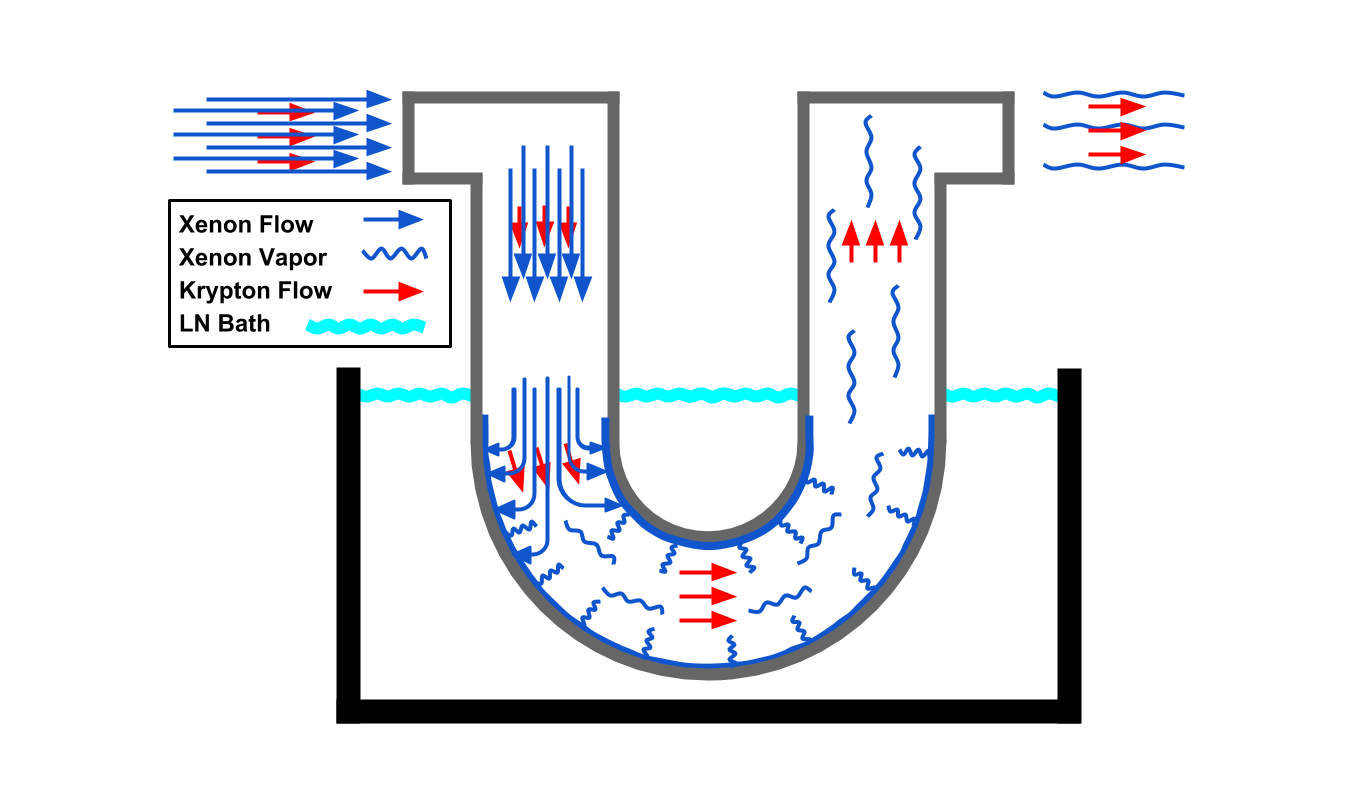
\includegraphics[width=\linewidth]{Figures/Cold_Trap_cartoon.png}
  \caption{Cartoon version of what happens during a cold trap analysis. }
  \label{fig:CTcartoon}
\end{figure}

\subsection{System Construction}
A cold trap sampling system should be laid out as described by figure \ref{fig:CTpid}. There will likely be additional transfer lines needed for collecting samples, recovering xenon, etc., but figure \ref{fig:CTpid} fully describes the plumbing necessary to analyze a sample of xenon.

\begin{figure}[h]
  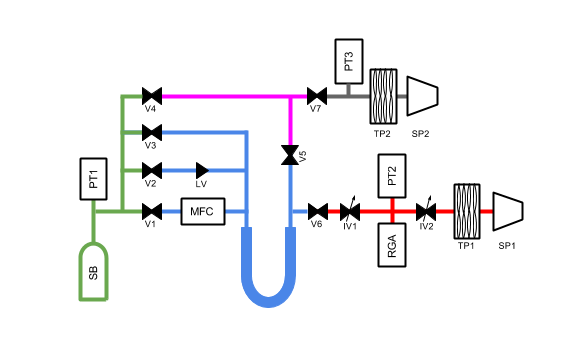
\includegraphics[width=\linewidth]{Figures/ColdTrap_diagram.png}
  \caption{Plumbing diagram of a general purpose cold-trap sampling system. The green section is referred to as the sample volume, the blue section is the cold trap volume, and the red section is the RGA volume. These are the sections used during analysis of a xenon sample. The pink section is the bypass line which serves two purposes. It is used to relieve pressure in the cold trap while the system is warming and acts as the access line to the pump-out turbo pump, TP2. }
  \label{fig:CTpid}
\end{figure}

The system should have 100\% metal-seals such as VCR or CF. Elastomer internals have the potential to become contaminated with krypton and destroy the sensitivity of the system and so should be limited.Traditionally, hardware used for this type of system is as follows:
\begin{itemize}
\item The plumbing should be entirely composed of UHP stainless steel.
\item The sample bottle, SB, is a \href{https://www.swagelok.com/en/product/Sample-Cylinders/DOT-Compliant}{1 gallon Swagelok DOT compliant sample cylinder}. 
\item The valves, V1 through V7 are some type of high purity shutoff valve. For automated systems, the \href{https://www.swagelok.com/en/product/Valves/Diaphragm-Sealed-Valves}{Swagelok DF series diaphragm valves} with pneumatic actuators are used. When possible, it is better to use the \href{https://www.swagelok.com/en/product/Valves/Bellows-Sealed}{Swagelok B series bellows valves} with the spherical copper stem tip option, since the DF series has a polymer seat, however these are more difficult to automate.
\item The sample pressure transducer is a capacitance manometer such as the \href{https://www.mksinst.com/product/category.aspx?CategoryID=72}{MKS Baratron} with a full scale of at least 3,000 Torr.
\item The leak valve, LV, is a metering valve.
\item The mass flow controller, MFC, should be metal sealed, and have a full range of about 10 SLM. The Celerity UNIT1660 is a good example. Although no longer in production, they are fairly easy to find used.
\item The cold trap itself is some UHP stainless steel plumbing that is bent or welded into a shape that allows it to be submerged in a liquid nitrogen bath. Currently, the optimal cold-trap geometry is a 1/2 inch ``stocking'' trap, as described in section \ref{sec:geometry}.
\item Traditionally IV1 has been a \href{https://www.swagelok.com/en/product/Valves/Bellows-Sealed}{Swagelok B series bellows valves} with the spherical copper stem tip option, however it's likely that the regulating stem tip would be better suited to the task. 
\item PT2 and PT3 are any cold cathode or inverted magnetron gauge that have an operating range of at least $10^{-8}$ to $10^{-4}$ Torr.
\item The residual gas analyzer, RGA, is the \href{http://www.thinksrs.com/products/RGA.htm}{SRS RGA200}.
\item IV2 needs to have a significantly lower impedance than IV1, so some type of 2.75" CF sealed all-metal vacuum valve should be used. A Varian UHV right angle valve, part No. 9515027 has been used in the past with good results.
\item TP1 and TP2 are turbo-molecular pumps with pumping speed of at least 70 liters per second. The Varian V70, V81, and V84 have all been used with good results.
\item SP1 and SP2 are the backing pumps for TP1 and TP2. They should be at least equivalent to the Agilent model SH110 scroll pump.
\end{itemize}  

\subsection{Operational Outline}
\label{sec:outline}
The exact steps required for a particular analysis can be quite complex, and some detailed example procedures can be found in  appendix \ref{ap:procedures}. A general outline of the operation of a cold trap sampling system is as follows:
\begin{enumerate}
\item A xenon sample is collected and stored in the sample volume until the beginning of analysis.
\item The system begins with all the valves closed.
\item  \label{step:analysis_start} The cold trap is immersed in a liquid nitrogen bath, and base layer of xenon ice is formed.
\item Baseline pressures are measured by the RGA by opening V6, exposing the RGA volume the the xenon ice vapor pressure present in the cold trap volume. Usually these baselines are established over a period of ten or more minutes.
\item \label{step:start_flow} Leaving V6 open, V1 or V2 is opened, allowing the xenon sample to freeze into the cold trap at a controlled flow rate. This will usually takes several minutes. 
\end{enumerate}
\noindent As described in figure \ref{fig:CTcartoon}, the xenon pressure at the RGA will remain constant during this step, but there will be a flow of krypton at the output of the cold-trap which will cause a rise in the krypton partial pressure in the RGA volume. It is this partial pressure pressure rise that will be analyzed to give the concentration of krypton in the xenon sample.
\begin{enumerate}[resume]
\item \label{step:stop_flow}After the sample volume has been exhausted, V1(2) will be closed, and the krypton partial pressure is allowed fall back to its prior value.
\end{enumerate}
\noindent At this point, the purity analysis of the xenon sample has been completed, but the system is not in a safe state. Only a microscopic amount of xenon has been pumped out through TP1, so the full mass of the xenon sample is frozen in the cold trap. If this is allowed to vaporize without proper precautions, the RGA and TP1 could be damaged by  over-pressure. It is therefore extremely important to isolate the RGA volume from the cold-trap volume before allowing the cold-trap to rise above liquid-nitrogen.
\begin{enumerate}[resume]
\item \label{step:analysis_stop} Close V6.
\end{enumerate}
\noindent If the sample mass was large enough, there could be enough xenon ice in the cold trap to damage the system instrumentation or even cause the plumbing system to rupture once it warms to the gas phase. This is why it is important to have rupture disks installed on the cold trap. To avoid damage to the system, the cold trap volume should be vented to the sample volume. Valve V3 provides a path from the input of the cold trap to the sample volume without the added impedance of the MFC or LV.
\begin{enumerate}[resume]
\item Open V3. 
\end{enumerate}
\noindent This is where the bypass line comes in. With a cold-trap made from 1/2" plumbing, it is likely that an ice blockage will form once the xenon flow has stopped. This ice blockage could cause a dangerous pressure differential between the input and output of the trap. By opening the bypass line, the output of the cold trap has a second path to the sample volume.
\begin{enumerate}[resume]
\item Open V4 and V5. 
\end{enumerate}

The system is now in a safe state and the cold trap can be allowed to warm back to room temperature. The remaining xenon can then be recovered or discarded as desired, after which the system should be pumped to vacuum before collecting the next sample. It is important to note that this pump-out should be done using TP2, since the RGA volume should be kept at vacuum except for maintenance. The bypass line, as configured, allows the cold-trap volume and sample volume to be pumped out independent of one another.

\subsection{Analysis Scheme}
The physical value we are interested in measuring is the concentration of an impurity, specifically krypton, in a sample of xenon gas. This value is typically referred to as $\Phi$ and cited in units of grams of krypton per gram of xenon. The calculation of $\Phi$ is done using the RGA partial pressure data collected between steps \ref{step:analysis_start} and \ref{step:analysis_stop} of the procedure outlined in section \ref{sec:outline}. An example of this data is shown in figure \ref{fig:RGAtrace}. 

\begin{figure}[h!]
  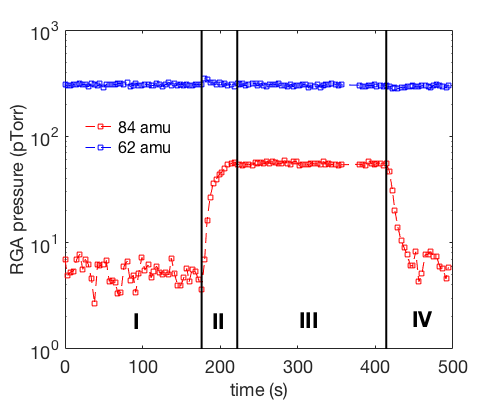
\includegraphics[width=\linewidth]{Figures/RGA_trace.png}
  \caption{The RGA-measured partial pressures of the 84 amu krypton peak and doubly ionized Xe-124 which appears as a peak at 62 amu. The four time intervals indicate: static baseline, rising Kr trace, steady-state Kr pressure, and post-flow Kr pressure fall.}
  \label{fig:RGAtrace}
\end{figure}

There are four distinct time-intervals in figure \ref{fig:RGAtrace} labelled I through IV. 
\begin{itemize}
\item I is the period of time after ice has been formed (step \ref{step:analysis_start}), but before the xenon flow has been started (step \ref{step:start_flow}). During this interval, both xenon and krypton traces should be constant; if they are trending or otherwise varying systematically, there is some problem that needs to be addressed before continuing. The average krypton pressure over this interval is used as the baseline value and will be subtracted from the analysis pressure. The average xenon pressure can be used as a measure of the RGA gain, since the physical xenon pressure will not change between sample analyses. 
\item II is the period of time after xenon flow has been started (step \ref{step:start_flow}), but before the krypton pressure has reached its equilibrium value. Given a long enough cold trap the krypton pressure during this step would fit a 1-exponential model, but the geometry of the cold trap can cause kinks in the trace. It is common for there to be a small transient effect in the xenon pressure as is seen here. This is likely due to the ice temperature increasing due to the added heat load from the flowing xenon. This transient effect can illicit an electronic response in the RGA baseline pressure which will mimmic a small krypton signal. The mitigation of this effect will be described in a later section.
\item III is the period of time during which the krypton pressure is at its equilibrium value. This equilibrium pressure is determined by the flow rate of the xenon, the sensitivity of the system, and $\Phi$.
\item IV is the period of time after the xenon flow has been stopped (step \ref{step:stop_flow}). During this period the krypton pressure will fall away exponentially before it eventually returns to the baseline value.
\end{itemize}

The shape of this signal can vary drastically depending on the concentration of krypton, the flow rate of xenon, the size of the xenon sample, the impedance of the system, and the physical geometry of the system. For a signal such as this, $\Phi$ can be extracted from these traces using a simple equation:
\begin{equation}
\label{eq:average_analysis}
PP_{Kr,eq}=CQ_{Xe}\Phi,
\end{equation}
where $PP_{Kr,eq}$ is the equilibrium krypton pressure at the RGA seen in region III, $C$ is a calibration constant which encapsulates the sensitivity of the system, and $Q_{Xe}$ is the flow rate of xenon into the cold trap. In high-sensitivity measurements, the sample volume will be exhausted before the krypton pressure equilibrates. In these cases we integrate equation \ref{eq:average_analysis} to give us:
\begin{equation}
\label{eq:int_analysis}
\Phi = \frac{1}{CV\Delta P_{Xe}}\int PP_{Kr}dt,
\end{equation}
where $V$ is the volume of the sample volume and $\Delta P$ is the total drop in xenon pressure in the sample volume. Also note that we have exchanged $PP_{Kr,eq}$ for the more general $PP_{Kr}$, which is the instantaneous krypton pressure in region II, III, or IV. In figure \ref{fig:linplot} we see that this method is linear in $\Phi$ even though we are including the non-equilibrium values of $PP_{Kr}$ in our analysis.
\begin{figure}[h!]
\centering
\begin{subfigure}{0.5\textwidth}
  \centering
  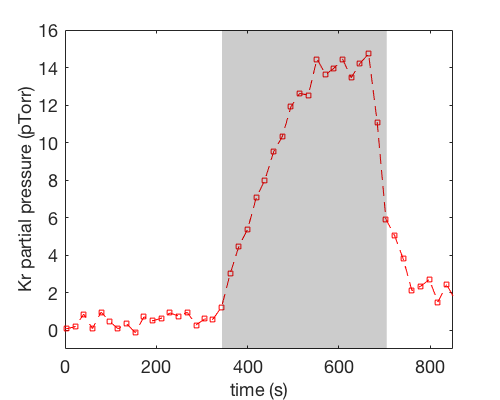
\includegraphics[width=\textwidth]{Figures/RGATrace_int.png}
  \caption{Sample RGA trace.}
\end{subfigure}%
\begin{subfigure}{0.5\textwidth}
  \centering
  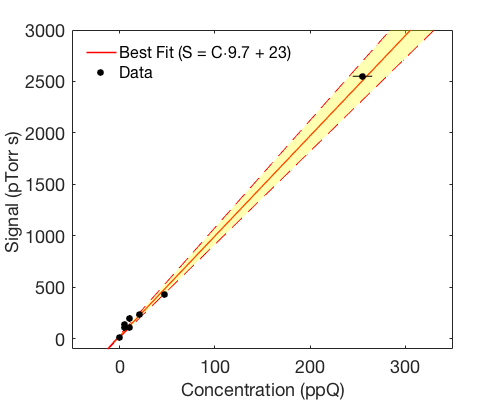
\includegraphics[width=\textwidth]{Figures/LinPlot0217.png}
  \caption{Linearity of analysis.}
\end{subfigure}
\caption{Linearity of the integration-style analysis described in equation \ref{eq:int_analysis}. The krypton signals used in these measurements never reached an equilibrium value.}
\label{fig:linplot}
\end{figure}

\subsection{Vacuum Equations}
In order to optimize the sensitivity of the cold-trap system, it is good to have an understanding of the basics of vacuum physics. A vacuum system can be analogized to an electrical circuit, with pressure taking the place of voltage, flow rate ($Q$) taking the place of current, and impedance ($Z$) taking the place if resistance.  This analogy gives us with the equation:
\begin{equation}
\label{eq:vaclaw1}
\Delta P = Q\cdot Z
\end{equation} 
Here, it is useful to define a new quantity, $S$, which is called the ``volumetric flow rate" or ``pumping speed''. $S$ is defined: 
\begin{equation}
\label{ep:volflow}
S \equiv Av = \frac{dV}{dt}, 
\end{equation}
where $A$ is the cross-sectional area of the pipe, and $v$ is the flow velocity, and $dV$ is the volume of gas which passes a point in the system in time $dt$. An effective pumping speed can be calculated for any point in the vacuum system through the equation:
\begin{equation}
\label{ep:vacimp}
1/S_{eff} = 1/S_{p}+Z_{total}, 
\end{equation}
where $S_{p}$ is the speed of the pump which is acting on the system, and $Z_{total}$ is the total impedance between the pump and the specified point in the system. By combining equation \ref{eq:volflow} with the definition of $Q$,
\begin{equation}
\label{ep:vacflow}
Q \equiv P\frac{dV}{dt},
\end{equation}
we are left with an extremely useful relation which relates the vacuum system parameters to the pressure at any point in the system\cite{vac_eq}:
\begin{equation}
\label{eq:vaclaw2}
Q \equiv P\cdot S_{eff}.
\end{equation}

The RGA has a maximum operating pressure of $1\times 10^{-6}$ Torr, although we have found that operating at slightly higher pressures is possible with minimal degradation of the CDEM. This being the case, we place the requirement that the absolute pressure at the RGA be less than about $2\times 10^{-5}$ Torr. When analyzing xenon samples with a concentration of about one part per million or less, the xenon partial pressure, $PP_{Xe}$,  will dominate the absolute pressure. $PP_{Xe}$ is the sourced by the vapor above the xenon ice in the cold trap bleeding out of the cold-trap volume, into the RGA volume. The vapor pressure of xenon ice at liquid nitrogen temperature is $P_{ICE}=1.8\times 10^{-3}$ Torr, and so needs to be reduced by a factor of about 100 or more between the cold-trap and the RGA\cite{vaporpressure}. This is done by choosing appropriate system impedances, specifically the impedance between the cold-trap and the RGA ($Z_1$) and the impedance between the RGA and TP1 ($Z_2$). $Z_1$ and $Z_2$ can be adjusted using IV1 and IV2, respectively. It should be noted here that xenon at $1.8\times 10^{-3}$ Torr and 77 Kelvin in a $0.5"$ diameter cold trap has a Knudsen number of 0.6, and so is actually in the intermediate gas flow regime rather than the molecular flow regime\cite{vac_eq}. For the purposes of this document, we will use the molecular flow approximation to motivate and direct our empirical investigations.

There are several compounding factors that come into play when deciding exactly what $PP_{Xe}$ should be. These will be discussed in later sections, so we will take it as given here that the sensitivity is optimized between $PP_{Xe}=5\times10^{-6}$ Torr, and $PP_{Xe}=2\times10^{-5}$ Torr, and is largely unaffected by deviations within this range. For the sake of simplicity, we will usually demand that $PP_{Xe}$ to be the default pressure that the system plumbing gives when IV1 and IV2 are maximized. For the system described above, the this pressure will be about $1\times 10^{-5}$ Torr. 

Returning to the vacuum equations we will see that although we have artificially defined $PP_{Xe}$, $Z_1$ and $Z_2$ are not fully determined by this choice. By using equations \ref{eq:vaclaw1} and \ref{eq:vaclaw2}, and the requirement that $PP_{Xe}=1\times 10^{-5}$ Torr, we place a constraint on the impedances:
\begin{equation}
\label{eq:xepres1}
Q_{Xe}=PP_{Xe}S_{RGA}=\frac{P_{ICE}-PP_{Xe}}{Z_1}\approx \frac{P_{ICE}}{Z_1},
\end{equation}
where $1/S_{RGA}=1/S_{TP1}+Z_2$. This gives,
\begin{equation}
\label{eq:impconstraint}
S_{RGA}\cdot Z_1= \frac{P_{ICE}}{PP_{Xe}} = 180.
\end{equation}
The exact numerical value of $S_{RGA}\cdot Z_1$ is less important than is the fact that for whatever amount $Z_1$ is increased, $S_{RGA}$ must be decreased proportionally in order to maintain the optimal $PP_{Xe}$. This means that $PP_{Xe}$ is held constant, regardless of $Z_1$.

The operating principle of cold-trap sampling is that while the xenon gets frozen into the cold-trap, the trace gasses, such as krypton pass through. Another way to put this is that at the output of the cold trap the xenon is frozen to a constant pressure, while krypton mass flow ($Q_{Kr}$) is conserved. In practice, the conservation is not perfect, so we add a throughput constant, $\alpha \equiv Q_{Kr}/Q_{Kr_0}$, where $Q_{Kr_0}$ is the flow rate into the cold trap. The physical basis of the throughput parameter is not known, but we have put great effort into characterizing it empirically. $Q_{Kr_0}$ is equal to the flow rate of xenon into the cold-trap ($Q_{Xe_0}$) times the concentration of krypton in the xenon sample, $\Phi_{Kr}$. Put together, we get the following equation: 
\begin{equation}
Q_{Kr}=\alpha Q_{Xe_0}\Phi_{Kr}.
\end{equation}
Plugging this into the vacuum equations, we can find the relationship between the parameter of interest, $\Phi_{Kr}$, and the measurable quantities, $Q_{Xe_0}$ and $PP_{Kr}$:
\begin{equation}
\label{eq:krpres1}
PP_{Kr}=\frac{\alpha}{S_{RGA}}\Phi_{Kr}Q_{Xe_0}.
\end{equation}
This relation shows the proportionality between partial pressure, and flow-rate times concentration that was found experimentally in \cite{sampling_doug} and \cite{sampling_dm}. By imposing the constraint from equation \ref{eq:impconstraint} we can see how altering the system impedance is expected to affect $PP_{Kr}$:
\begin{equation}
\label{eq:krpres2}
PP_{Kr}=\frac{\alpha}{180}Z_{1}\Phi_{Kr}Q_{Xe_0}.
\end{equation}
This equation yields an important insight into the optimization of a cold-trap sampling system. By holding $PP_{Xe}$ constant through adjusting $S_{RGA}$, the krypton partial pressure can be increased by increasing $Z_1$, which means that a larger signal can be achieved using the same sample size of xenon.


\section{System Parameters and Optimization}
There are several knobs to turn that affect a cold-trap sampling system's response to krypton. In general these are:
\begin{enumerate}
\item RGA parameters
\item Xenon flow rate and duration
\item System impedances
\item System geometry
\end{enumerate}
These settings all have individual effects on the sensitivity of the sampling system, but also interact with each other in nontrivial ways that must be understood empirically in order to maximize the system response to krypton.

\subsection{RGA Parameters} 
There is a long list of internal RGA parameters which should be understood before operating a cold trap system. These can be found in chapter 6 of the \href{http://www.thinksrs.com/downloads/PDFs/Manuals/RGAm.pdf}{RGA manual}. The two parameters that have the greatest effect on the sensitivity to krypton are the noise floor and the high-voltage setting of the continuous dynode electron multiplier (CDEM). 

The noise floor sets the scan speed of the RGA; the lower the noise floor setting, the longer the RGA will spend integrating current on a single mass point. The practical effects are threefold. The obvious first implication is that with a low noise floor, it will take much longer to to collect a single data point. At a noise floor setting of 0 the RGA will sit on a mass point for about 5 seconds, and at a noise floor setting of 3 it will sit for less the 0.5 seconds per mass. For high-sensitivity analysis, it is better to have the noise floor set as low as possible, which will give you fewer data points which have a smaller variance. This will reduce the amount of time spent communicating with the RGA, as well as the amount of down time between communications. 

{\color{red}At higher noise floors, there tends to be an offset in the baseline. While we usually try to account for this by using baseline-subtracted pressures in purity calculations, it is possible that the shifted baseline is not additive to the pressure signal. This is indicated by the krypton signal in the LUX run04 data decreasing artificially. There is also evidence from the SLAC system that the baseline is not strictly additive to a physical pressure signal.}

Setting the voltage on the CDEM is a balancing act. Increasing the voltage increased the signal amplification. Above a certain CDEM voltage, however, the random fluctuations in the RGA baseline rise faster than the gain, and if the voltage is set too high, the xenon ice vapor pressure will begin saturate the CDEM, degrading and possibly damaging it. The CDEM voltage should be high enough that the largest xenon peaks such as 132 and 133 should be at saturation but not so high that the doubly ionized peaks such as 66 amu saturate. 

\begin{figure}[h]
  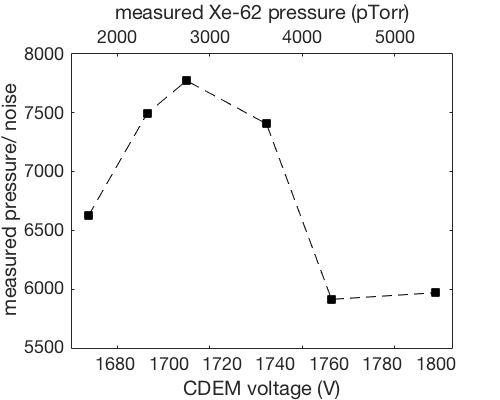
\includegraphics[width=\linewidth]{Figures/CDEM_gain_noise.png}
  \caption{RGA sensitivity as a function of CDEM voltage. }
  \label{fig:CTpid}
\end{figure}

The health of the CDEM can be tracked using one of the xenon ice peaks, assuming the MG and SP parameters are not changed. MG is the CDEM gain factor and SP is the mass sensitivity factor used to convert the RGA current to partial pressure. The physical values may change over time, but the parameter stored in the RGA memory will not change unless a head-calibration is run. In particular, as the CDEM degrades, the gain will fall. A drift in the gain will bee seen most easily as a drop in the measured xenon ice pressure. Since the vapor pressure of xenon ice at 77 Kelvin is physically constant, if this pressure reading drops, it indicates that the gain has dropped. To maintain the CDEM gain, the xenon peak at 62 amu should be monitored. Whenever this value drops, the voltage should be increased until the pressure returns to its initial value.

\subsection{Flow Rate}

\begin{figure}[h]
  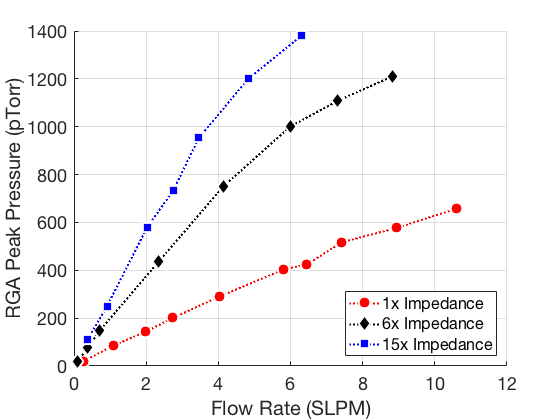
\includegraphics[width=\linewidth]{Figures/FlowResponse.png}
  \caption{Peak krypton RGA pressure as a function of flow rate.  }
  \label{fig:flowresponse1x}
\end{figure}

\subsection{Impedance}

\subsection{System Geometry}
\label{sec:geometry}

\subsection{Ice Formation Procedure}

\section{Calibrations}
Once the system has been optimized using a largely arbitrary mixture of xenon and krypton, the next key step is to measure the response of the system to a series of mixtures referred to as calibration xenon which have well known concentrations of krypton. Once this response is known, the system can be used to measure concentrations of unknown mixtures. To this end, the preparation of a mixture of xenon and krypton with a well known concentration is essential.

\subsection{Preparation of Calibration Xenon}
The first ingredient in the preparation of this mixture is extremely pure xenon. This is obtained by using the cold trap system itself to clean a small amount of stock xenon. As was explained previously, the cold trap analysis works because all but a microscopic amount of xenon is retained by the cold trap, while gasses such as krypton pass through largely unaffected. This means that the xenon that remains in the cold trap after an analysis has significantly lower krypton content than before the analysis. Depending on the system parameters, the post-run xenon will contain as little as $1/15^{\textrm{th}}$ the krypton as the pre-run xenon. Using the system described by figure \ref{fig:SLACpid}, it takes about 3 hours to purify 100g of typical stock xenon with a concentration of 1 part in $10^{9}$ down to $< 1$ part in $10^{15}$, 


\begin{figure}[h]
  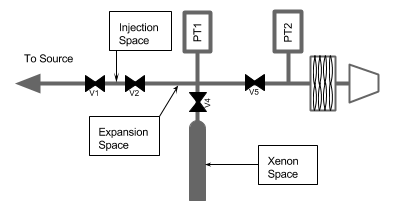
\includegraphics[width=\linewidth]{Figures/Mixing_diagram.png}
  \caption{Plumbing diagram of a generalized mixing system. }
  \label{fig:mixpid}
\end{figure}

Once the xenon has been cleaned it is transferred to an appropriate mixing system, described by figure \ref{fig:mixpid}. The relative volumes of this system must be extremely well known, so they are measured using volume sharing. First the full system, including injection, expansion, and xenon volumes, is filled with roughly 2000 torr of xenon as measured by pressure transducer 1. Then the expansion volume is pumped to vacuum, leaving a well known pressure in both the injection and xenon volumes. Valve 4 is opened to expose the xenon within the xenon volume to the expansion volume. The resulting pressure on PT1 gives the expansion volume relative to the xenon volume. Through the ideal gas law, when temperature is constant and mass is conserved, pressure times volume will remain constant:
\begin{equation}
P_{1}V_{1} = P_{2}V_{2}
\end{equation}
Therefore, the size of the expansion volume relative to the xenon volume can be calculated using:
\begin{equation}
\frac{\textrm{Expansion Vol.}}{\textrm{Xenon Vol.}} = P_{1}/P_{2}-1.
\end{equation}
Similarly, the relative size of the injection volume is found by expanding the known pressure within the injection volume into the expansion volume. 

To prepare the calibration xenon, the injection volume is filled to some known pressure with pure krypton. The krypton is then opened to the expansion volume in order to reduce the pressure, and then the expansion volume is pumped out using a the turbo-pump until PT2 reads $<1\times10^{-6} \textrm{ torr}$. This expansion is repeated until the desired krypton pressure is reached. After the final expansion volume pump-out, the xenon volume is opened to the injection volume, and the new xenon/krypton mixture is frozen back into the xenon volume using liquid nitrogen. The krypton concentration ($\Phi_{Kr}$) of the calibration xenon in grams krypton per grams xenon is given by:
\begin{equation}
\Phi_{Kr} = \frac{\alpha^{N}P_{Kr}(\textrm{Injection Vol.})\rho_{Kr} }{P_{Xe}(\textrm{Xenon Vol.})\rho_{Xe}},
\end{equation}
where the expansion ration, $\alpha$, is given by (Injection Vol.)/(Injection Vol. + Expansion Vol.), $N$ is the number of expansions, $P_{Kr}$ and $P_{Xe}$ are the krypton and xenon pressures initially injected into the system, and $\rho_{Kr}$ and $\rho_{Xe}$ are the krypton and xenon gas densities.

The injection pressure must be kept above 0.01 torr to ensure the krypton remains above the molecular flow regime. This sets a lower limit on the concentration of calibration xenon that can be produced through this method. With an injection volume of 5cc and a xenon volume of 4000cc, the lowest concentration than can be produced from pure krypton is about 5 PPB. In order to produce calibration xenon with smaller concentrations, the pure krypton is replaced with the PPB level calibration xenon, which is diluted into clean xenon through the same process outlined in the previous paragraph.

\subsection{Calibration Procedure}


\section{Sensitivity Demonstration}




\appendix
\section{Sample Procedures}
\label{ap:procedures}



\bibliography{main}{}
\bibliographystyle{Science}

\end{document}




















